\documentclass{ics-paper}

\usepackage{fancyhdr}
\usepackage[ruled]{algorithm2e}
\renewcommand{\headrulewidth}{0pt}
\fancypagestyle{firstpage}{
  \fancyhf{}
  \fancyhead[C]{\normalsize{Lab 3 in CSCI 59000 HPC Spring 2017 }} 
}

\graphicspath{ {images/} }


\author{Feng Li}
\date{Feb 28, 2017}

\title{\textbf{\sffamily Implementation of SUMMA Algorithm using MPI}}

\begin{document}

\maketitle
\thispagestyle{firstpage}

\begin{abstract}
In the first and second lab, only one process was used to solve the dgemm problem. By using different optimization techniques, the best gflops of sequential implementation is still below 10. By using MPI(Message Passing Interface), a multi-process algorithm- ‘SUMMA’ is implemented in this lab. Scalalibity and efficiency of this implementation is also examined in Big Red II. 
\end{abstract}

\section{Introduction}
In lab 1 and lab2, we compared the performance of naive dgemm algorithm with optimized dgemm with blocking and loop-unrolling techniques. Though these optimization techniques can improve either space or time locality of the sequential program, they didn't utilize the powerful computing capacity of nowadays HPC systems. Thus in this lab, we use SUMMA algorithm, which is distributed and scalable for large matrix size, to demonstrate how to use multi-processing in HPC systems to accelerate matrix multiplication problems. 
\subsection{MPI}
MPI(\cite{gropp1996high}) is a communication protocol for parallel computing. Both point-to-point and collective communication paradigms are supported. The goal of this protocol is to provide a standard for writing message passing programs. Languages supported by MPI are C, C++, FORTRAN, etc. It's not a IEEE or ISO standard, but currently is the 'industry standard' in high performance computing fields. This protocol is highly portable, though there are different implementations from various vendors, they all provide high performance and scalability.
\subsection{SUMMA}
SUMMA(\cite{van1997summa}) is a distributed solver for matrix multiplication problems. It is used in Scalapac and other related libraries. Original algorithm of SUMMA is more general and complexed, however in this lab only special cases are considered(eg. matrix is square, matrix size is dividable by block size, etc.) Details of SUMMA algorithm will be in section \ref{sec:algo}.
\section{algorithm and implementation}
The idea of SUMMA algorithm can be shown when we rearrange the order loops in
naive dgemm algorithm. Using the order kij, the code is as following:
\begin{algorithm}
	\For{$k=1$ to $n$}{
		\For{$i=1$ to $n$}{
			\For{$j=1$ to $n$}{
				$C(i,j) += A(i,k)*B(k,j)$ \;
			}
		}
	}
	\caption{rearranged naive dgemm}
\end{algorithm}

This can be further abbreviated to: 
\begin{algorithm}
	\For{$k=1$ to $n$}{
		C = C + A(:,k)*B(k,:)\;
	}
	\caption{simplified version}
\end{algorithm}

The operation in the loop will be a multiplication of one column from A and one row from B, which will produce a $n*n$ matrix. To distribute the computation to different processes, each process will has its own partition of matrix A, B and C. Also in each iteration, the processes which owns part of column $A(:,k)$ will send that partial column to other processes in the same row; in the same way, the processes which owns part of row $B(k,:)$ will send that partial row to other processes in the same column. A pseudo code is shown is Algorithm \ref{algo:summa}.

\begin{algorithm}
	\SetAlgoLined
	\KwIn{\\
		\Indp $A_{sub}$, $B_{sub}$, $C_{sub}$, sub matrix \\
		 $N$, matrix size \\
		 $N_{sub}$, sub-matrix size \\
		 b, block size \\
		 nprocs, number of processes \\
		 rank,  my rank
	}


	\KwOut{\\
		\Indp $C_{sub}$, output matrix}
	\textbf{Begin} \\
	$N_{sub}=N/sqrt(nprocs)$ \;
	
	$procs\_side=N/sqrt(nprocs)$ \;
	$my\_row = rank/procs\_side$\;
	$my\_col = rank\%procs\_side$ \;
	
	generate row communicator \textbf{row\_comm} using $my\_row$ \;
	generate col communicator \textbf{col\_comm} using $my\_col$ \;

	allocate space for column block $colblock$, size $N_{sub}*b$ \;
	allocate space for row block $rowblock$, size $b*N_{sub})$ \;

	\For{$k=0;k<N/b;k++$}{
		// check wheter i have the column \;
		\If{$my\_col == k*b/N_{sub}$}{
			store the block of data into $colblock$
		}
		// broadcast in the row direction\\
		Mpi\_Bcast(col\_block, $ k*b/N_{sub}$, $row\_comm$)\;

		// check wheter i have the row \;
		\If{$my\_row == k*b/N_{sub}$}{
			store the block of data into $rowblock$
		}
		// broadcast in the column direction\\
		Mpi\_Bcast(row\_block, $ k*b/N_{sub}$, $col\_comm$)\;
		// update local C submatrix
		$C += colblock*rowblock$
	}
	
	
	\textbf{End} 
	\caption{SUMMA algorithm}
	\label{algo:summa}
\end{algorithm}

As described in algorithm \ref{algo:summa}, two subcommunicators(row communicator and column communicator) are generated using the row id and column id, respectively. In each of $k$ outer loop, each process will check whether it has the column block or row block to be send to other processes. There is no explicit send or receive function involved. Instead mpi\_bcast is used to copy the row/column bock to other processes who are in the same row/column.Since mpi\_bcast uses tree structures to accerlate the communication among all the processes in the same communicator, it is more efficient than just calling mpi\_send/mpi\_recv repeatedly.
\label{sec:algo}

\section{Experiment Results and Discussion}
\subsection{experiment configurations}
The input matrix A and B are generated from root matrix and then divided and distributed to other processes. A timer is added in each process to record the elapsed time used to finish all iterations. The resulting gflops is calculated using the average elapsed time from all processes. To verify the correctness of SUMMA algorithm, after root process gathers all the partial results from other processes, it will compare the results with that from Libsci blas routines.
\subsection{best performance using different nodes}

First experiment is to show how overall performance changes when we increase number of processes for various matrix sizes. From the result shown in figure \ref{fig:totalflops}, it's clear that four all the cases, more processes will produce higher total gflops. This is straightforward since more cpus are used during computation thus larger throughput can be delivered.
\begin{figure}
	
	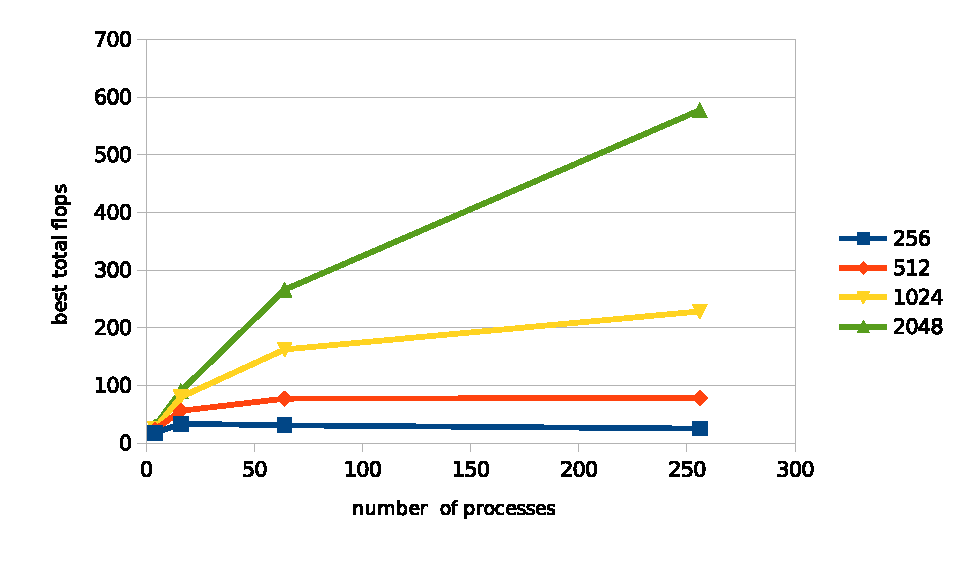
\includegraphics[height=1.5in, width=3in]{total_flops}
	\caption{total gflops, different colors represents using different matrix sizes}
	\label{fig:totalflops}
\end{figure}
However the increase in total glops is not linear. When process number is doubled, total performance doesn't increase by two times.To have a closer look at this, the glops per process is shown in figure \ref{fig:scale}, which suggests that when number of nodes keep increasing, the actually efficiency of parallel algorithm decreases significantly.The best gflops per process, $7.19$, is achieved when matrix size if 2048 and using 4 processes with block size 1048(same with sub-matrix size). Since the peak gflops of each core is 10 gflops. The best efficiency of 71.9, which is rather high. It should be mentioned that though only matrix sizes no larger than 2048 are tested, from figure \ref{fig:scale}, it's pretty clear that matrix with size larger than 2048 will produce even higher best gflops per process.

\begin{figure}
	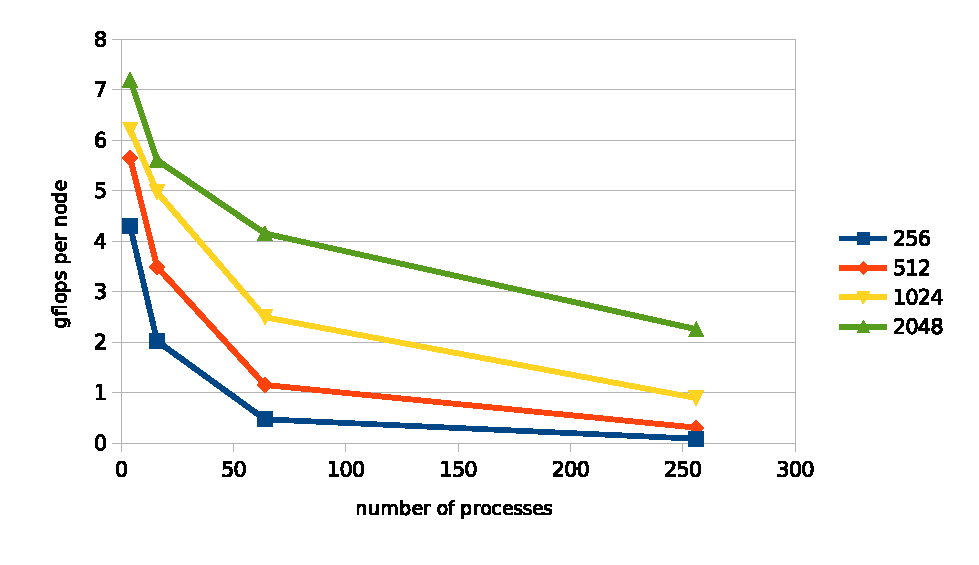
\includegraphics[height=1.5in, width=3in]{scale}
	\caption{gflops per process,different colors represents using different matrix sizes}
	\label{fig:scale}
\end{figure}


\label{sec:3.1}
\subsection{block size}
\begin{figure}
	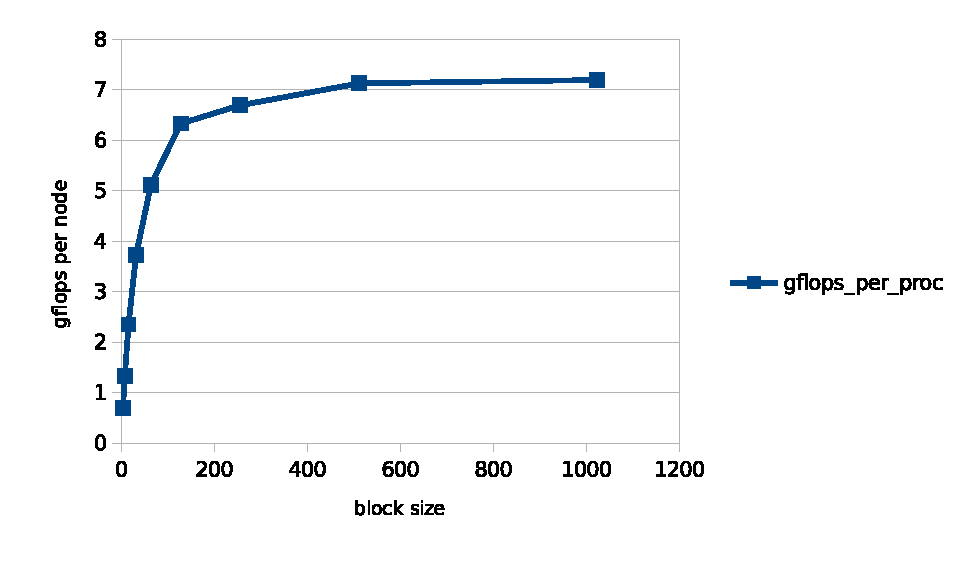
\includegraphics[height=1.5in, width=3in]{blocksize}
	\caption{total gflops, different colors represents using different number of processes}
	\label{fig:blocksize}...
\end{figure}
To examine the correlation between block size and efficiency of the SUMMA implementation, in this experiment fixed matrix size and process numbers are used in this part \ref{sec:3.1}, which are 2048 and 4, respectively. Result is show in figure \ref{fig:totalflops}, where it's obvious that gflops will increase when block size goes up. This is reasonable since with larger block size, the overhead of MPI communication is relatively smaller.
However, the glops per process doesn't increase any more after block size becomes even larger. The reason is that larger block size makes the dgemm subroutine more resource demanding.

\section{conclusion}
To conclude, SUMMA algorithm is correctly implemented using MPI. When more processes are used the algorithm can deliver significantly higher gflops compared with sequential implementation. However the efficiency of summa algorithm will decrease with larger number of processes because there will be more messages. For the block size, larger block sizes tend to give better efficiency since more data is transferred in each MPI message.

\bibliographystyle{plain}
\bibliography{references}

\end{document}
